\chapter{Funciones a optimizar}

En este capítulo se presenta el núcleo experimental del proyecto: el análisis comparativo de cinco métodos de optimización aplicados a siete funciones de prueba. Se ha elegido un conjunto variado de funciones de prueba, considerando aspectos como la complejidad de su superficie, la presencia de múltiples óptimos locales, la dimensión del problema y la sensibilidad a las condiciones iniciales. Cada función ha sido seleccionada con el objetivo de cubrir un amplio espectro de escenarios que suelen encontrarse en problemas de optimización del mundo real.

\section{Función de Bohachevsky} % 17

La función de Bohachevsky está definida como:
$$f_1(\mathbf{x}) = x_1^2 + 2x_2^2 - 0.3 \cos(3\pi x_1) - 0.4\cos(4\pi x_2) + 0.7.$$
Está función la evaluaremos en $x_i \in [-100, 100]$, para $i = 1, 2$. En \citep{sfuoptimization}, se menciona que el mínimo global está en $\mathbf{x}^* = (0, 0)$ y al evaluarlo en la función se obtiene $f_1\left(\mathbf{x}^*\right) = 0$.
\begin{figure}[H]
    \centering
    \subfloat[Gráfica de la función de Bohachevsky]{
    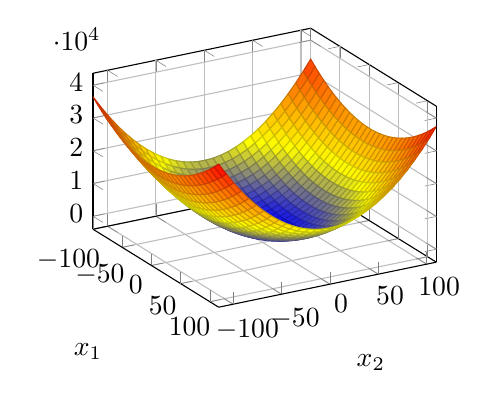
\begin{tikzpicture}
        \begin{axis}[
            xlabel=$x_1$,
            ylabel=$x_2$,
            xtick distance=50,
            ytick distance=50,
            ztick distance=10000,
            grid=major,
            domain=-100:115,
            y domain=-115:110,
            view={60}{30},
            width=0.49\textwidth,
        ]
            \addplot3[surf, samples=30] {x^2 + 2*y^2 - 0.3*cos(deg(3*pi*x)) - 0.4*cos(deg(4*pi*y)) + 0.7};
        \end{axis}
    \end{tikzpicture}
    }
    \subfloat[Curvas de nivel de la función de Bohachevsky]{
    \begin{tikzpicture}
        \begin{axis}[
            xlabel=$x_1$,
            ylabel=$x_2$,
            domain=-100:100,
            y domain=-100:100,
            view={0}{90},
            width=0.49\textwidth,
        ]
        \addplot3[contour gnuplot={
            levels={0, 500, 1000, 2000, 4000, 8000, 12000, 16000, 20000, 24000, 28000, 30000},
            labels=false,},
            thick,
            samples=30] gnuplot {x**2 + 2*y**2 - 0.3*cos(3*pi*x) - 0.4*cos(4*pi*y) + 0.7};
        \end{axis}
    \end{tikzpicture}
    }
    \caption{}
\end{figure}

\newpage\noindent
Al correr nuestros programas, obtenemos la siguiente tabla:
\begin{table}[H]
    \begin{NiceTabular}{ccccc}[hvlines-except-borders,cell-space-limits=5pt,rules={color=white,width=1pt}]
        \CodeBefore
        \rowcolor{cw0!80}{1}
        \rowcolors{2}{cw2!70!white}{cw1!30!white}
        \Body
        \RowStyle[color=white]{}
        \RowStyle{\bfseries}
        Método & Iteraciones & Punto óptimo & Función evaluada & Error \\
        Máxima Pendiente & $82$ & $\left(-4.5596 \times 10^{-9}, 4.1631 \times 10^{-10}\right)$ & $0.000000$ & $0.18034$ \\
        Método de Newton & $34$ & $(0.00,0.00)$ & $0.00$ & $0.00$ \\
        Cuasi-Newton Rango 1 & $13$ & $(-0.0000, -0.0000)$ & $0.0000$ & $0.0000$ \\
        Gradientes Conjugados & $279$ & $(0.0000, 0.469528)$ & $0.469882$ & $0.039030$ \\
        Hooke-Jeeves & $65$ & $(-0.000000, -0.000000)$ & $0.000000$ & $0.000000$
    \end{NiceTabular}
    \caption{Resultados de la función de Bohachevsky usando \emph{multistart} con $N = 2500$}
\end{table}

El método \textbf{Cuasi-Newton de Rango 1} demuestra ser el más eficiente. Con tan solo \textbf{13 iteraciones}, converge al óptimo teórico $(0,0)$, obteniendo un valor de función y un error residual nulos.

Los métodos de \textbf{Newton} y \textbf{Hooke-Jeeves} también alcanzan el óptimo exacto con un error de cero. Sin embargo, requieren un esfuerzo computacional considerablemente mayor, con 34 y 65 iteraciones respectivamente, lo que los hace menos eficientes en comparación con el método Cuasi-Newton.

Por otro lado, \textbf{Máxima Pendiente} emplea 82 iteraciones con error 0.18034, frente a las 279 iteraciones y error 0.03903 de \textbf{Gradientes Conjugados}; aunque es más rápida, su solución se aleja más del óptimo global.

\section{Función de Booth} % 24

La función de Booth está definida como:
$$f_1(\mathbf{x}) = (x_1 + 2x_2 - 7)^2 + (2x_1 + x_2 - 5)^2.$$
Está función la evaluaremos en $x_i \in [-10, 10]$, para $i = 1, 2$. En \citep{sfuoptimization}, se menciona que el mínimo global está en $\mathbf{x}^* = (1, 3)$ y al evaluarlo en la función se obtiene $f_1\left(\mathbf{x}^*\right) = 0$.
\begin{figure}[H]
    \centering
    \subfloat[Gráfica de la función de Booth]{
    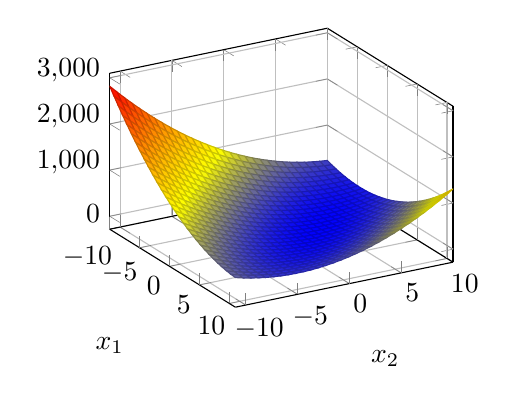
\begin{tikzpicture}
        \begin{axis}[
            xlabel=$x_1$,
            ylabel=$x_2$,
            xtick distance=5,
            ytick distance=5,
            ztick distance=1000,
            grid=major,
            domain=-10:11,
            y domain=-11:10,
            view={60}{30},
            width=0.49\textwidth,
        ]
            \addplot3[surf, samples=30] {(x + 2*y - 7)^2 + (2*x + y - 5)^2};
        \end{axis}
    \end{tikzpicture}
    }
    \subfloat[Curvas de nivel de la función de Booth]{
    \begin{tikzpicture}
        \begin{axis}[
            xlabel=$x_1$,
            ylabel=$x_2$,
            xtick distance=2,
            ytick distance=2,
            domain=-10:10,
            y domain=-10:10,
            view={0}{90},
            width=0.49\textwidth,
        ]
        \addplot3[contour gnuplot={
            levels={0, 5, 10, 20, 30, 40, 50, 70, 90, 120},
            labels=false,},
            thick,
            samples=30] gnuplot {(x + 2*y - 7)**2 + (2*x + y - 5)**2};
        \end{axis}
    \end{tikzpicture}
    }
    \caption{}
\end{figure}

\newpage\noindent
Al correr nuestros programas, obtenemos la siguiente tabla:
\begin{table}[H]
    \begin{NiceTabular}{ccccc}[hvlines-except-borders,cell-space-limits=5pt,rules={color=white,width=1pt}]
        \CodeBefore
        \rowcolor{cw0!80}{1}
        \rowcolors{2}{cw2!70!white}{cw1!30!white}
        \Body
        \RowStyle[color=white]{}
        \RowStyle{\bfseries}
        Método & Iteraciones & Punto óptimo & Función evaluada & Error \\
        Máxima Pendiente & $21$ & $(1.000000, 3.000000)$ & $0.000000$& $4.4658 \times 10^{-7}$ \\
        Método de Newton & $2$ & $(1.000000, 3.000000)$ & $0.000000$ & $0.000000$ \\
        Cuasi-Newton Rango 1 & $5$ & $(1.000000, 3.000000)$ & $0.000000$ & $0.000000$ \\
        Gradientes Conjugados & $2$ & $(1.000000,3.000000)$ & $0.000000$ & $0.050401$ \\
        Hooke-Jeeves & $47$ & $(1.000000, 3.000000)$ & $0.000000$ & $0.000000$
    \end{NiceTabular}
    \caption{Resultados de la función de Booth usando \emph{multistart} con $N = 2500$}
\end{table}

Como se observa en la tabla, todos los métodos convergen al óptimo $(1, 3)$ con un valor de función de cero. Para evaluar su rendimiento, usamos dos métricas: la eficiencia, medida por el número de iteraciones hasta la convergencia, y la precisión, cuantificada por el error residual, que debe tender a cero para garantizar la exactitud.

En el grupo de métodos que alcanzaron un error nulo, el \textbf{Método de Newton} destaca como el más eficiente, requiriendo únicamente \textbf{2 iteraciones} para converger. Le sigue de cerca el método \textbf{Cuasi-Newton de Rango 1}, que también logra una precisión perfecta en tan solo 5 iteraciones, consolidándose como una excelente alternativa. Aunque el método de \textbf{Hooke-Jeeves} también encuentra la solución exacta, su costo computacional es significativamente mayor, con 47 iteraciones.

Respecto a los métodos con un error residual, se presenta un interesante compromiso entre velocidad y precisión. El método de \textbf{Gradientes Conjugados} es tan rápido como el de Newton, llegando al óptimo en solo \textbf{2 iteraciones}, pero a expensas de la precisión, ya que registra el error más alto de todos. Por su parte, \textbf{Máxima Pendiente} (con Armijo) requiere 21 iteraciones y finaliza con un error muy pequeño, aunque no nulo.

En conclusión, para la función de Booth, el \textbf{Método de Newton} es indiscutiblemente superior, ofreciendo una combinación inmejorable de velocidad y exactitud. Si bien \textbf{Gradientes Conjugados} iguala su velocidad, su considerable error lo hace menos fiable. Los métodos de \textbf{Hooke-Jeeves} y, en menor medida, \textbf{Máxima Pendiente} resultan ser los que demandan un mayor esfuerzo computacional.

Para problemas similares a la función de Booth, conviene valorar no solo la velocidad sino también el coste de calcular la Hessiana. El Método de Newton es muy rápido y preciso, pero su necesidad de la matriz Hessiana puede volverse prohibitiva en alta dimensión. En cambio, Gradientes Conjugados y Cuasi-Newton reducen el esfuerzo por iteración al aproximar la curvatura, sacrificando algo de exactitud, y resultan más adecuados cuando no se dispone de derivadas segundas o se trabaja a gran escala.

\section{Función Goldstein-Price} % 40

La función Goldstein-Price está definida como:
\begin{align*}
    f(\mathbf{x}) & = \left[1 + \left(x_1 + x_2 + 1\right)^2 \left(19 - 14x_1 + 3x_1^2 - 14x_2 + 6x_1 x_2 + 3x_2^2\right)\right] \\
    & \hspace{3cm} \times \left[30 + \left(2x_1 - 3x_2\right)^2 \left(18 - 32x_1 + 12x_1^2 + 48x_2 - 36x_1 x_2 + 27x_2^2\right)\right].
\end{align*}
Está función la evaluaremos en $x_i \in [-2, 2]$, para $i = 1, 2$. En \citep{sfuoptimization}, se menciona que el mínimo global está en $\mathbf{x}^* = (0, -1)$ y al evaluarlo en la función se obtiene $f\left(\mathbf{x}^*\right) = 3$.
\begin{figure}[H]
    \centering
    \subfloat[Gráfica de la función Goldstein-Price]{
    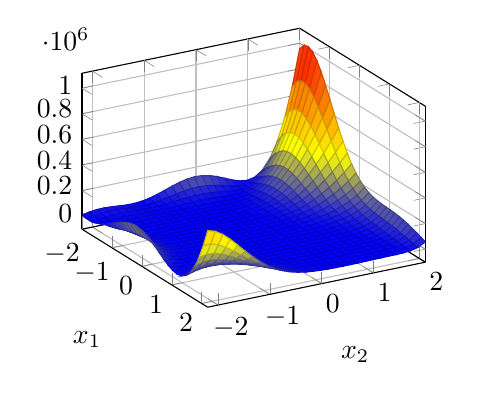
\begin{tikzpicture}
        \begin{axis}[
            xlabel=$x_1$,
            ylabel=$x_2$,
            xtick distance=1,
            ytick distance=1,
            ztick distance=200000,
            grid=major,
            domain=-2:2.2,
            y domain=-2.2:2,
            view={60}{30},
            width=0.49\textwidth,
        ]
            \addplot3[surf, samples=30] {(1 + (x + y + 1)^2 * (19 - 14*x + 3*x^2 - 14*y + 6*x*y + 3*y^2)) * (30 + (2*x - 3*y)^2 * (18 - 32*x + 12*x^2 + 48*y - 36*x*y + 27*y^2))};
        \end{axis}
    \end{tikzpicture}
    }
    \subfloat[Curvas de nivel de la función Goldstein-Price]{
    \begin{tikzpicture}
        \begin{axis}[
            xlabel=$x_1$,
            ylabel=$x_2$,
            xtick distance=1,
            ytick distance=1,
            domain=-2:2,
            y domain=-2:2,
            view={0}{90},
            width=0.49\textwidth,
        ]
        \addplot3[contour gnuplot={
            levels={50, 100, 200, 500, 1000, 2000, 4000, 8000},
            labels=false,},
            thick,
            samples=30] gnuplot {(1 + (x + y + 1)**2 * (19 - 14*x + 3*x**2 - 14*y + 6*x*y + 3*y**2)) * (30 + (2*x - 3*y)**2 * (18 - 32*x + 12*x**2 + 48*y - 36*x*y + 27*y**2))};
        \end{axis}
    \end{tikzpicture}
    }
    \caption{}
\end{figure}

\noindent Al correr nuestros programas, obtenemos la siguiente tabla:
\begin{table}[H]
    \begin{NiceTabular}{ccccc}[hvlines-except-borders,cell-space-limits=5pt,rules={color=white,width=1pt}]
        \CodeBefore
        \rowcolor{cw0!80}{1}
        \rowcolors{2}{cw2!70!white}{cw1!30!white}
        \Body
        \RowStyle[color=white]{}
        \RowStyle{\bfseries}
        Método & Iteraciones & Punto óptimo & Función evaluada & Error \\
        Máxima Pendiente & $11$ & $\left(3.2909 \times 10^{-10}, -1\right)$ & $3.000000$ & $0.000000$\\
        Método de Newton & $11$ & $(-0.000000, -1.000000)$ & $4.000000$ & $0.000000$ \\
        Cuasi-Newton Rango 1 & $11$ & $(-0.000000, -1.000000)$ & $3.000000$ & $0.000000$ \\
        Gradientes Conjugados &$648$ &$ (-0.041638, -1.010081)$ & $3.405280$ & $0.235384$ \\
        Hooke-Jeeves & $29$ & $(0.000000, -1.000000)$ & $3.000000$ & $0.000000$ \\
    \end{NiceTabular}
    \caption{Resultados de la función Goldstein-Price usando \emph{multistart} con $N = 2500$}
\end{table}

Observamos que los métodos de \textbf{Máxima Pendiente}, \textbf{Newton} y \textbf{Cuasi-Newton Rango 1} convergen en solo 11 iteraciones, mientras que \textbf{Hooke–Jeeves} requiere 29. Sin embargo, solo Máxima Pendiente y Cuasi-Newton Rango 1 alcanzan el valor correcto de la función. El Método de Newton, a pesar de localizar exactamente el óptimo, reporta $f  =4$, lo cual sugiere un posible error en la evaluación de la función.

Por el contrario, los \textbf{Gradientes Conjugados} resultan claramente ineficientes: tras 648 iteraciones no llegan al óptimo global, convergiendo a $(-0.0416, -1.0101)$ con $f \approx 3.4053$ y un error residual significativo. Este comportamiento denota sensibilidad a la forma del paisaje y un coste computacional excesivo.

En conclusión, los métodos más robustos para Goldstein–Price son \textbf{Máxima Pendiente} y \textbf{Cuasi-Newton Rango 1}, que equilibran rapidez (11 iteraciones) y exactitud en la evaluación de la función. Hooke–Jeeves ofrece convergencia exacta pero a mayor costo iterativo, mientras que Newton, pese a su velocidad, requiere revisar su implementación de la función, y Gradientes Conjugados no resulta recomendable debido a su elevado número de iteraciones y error final.  

\newpage

\section{Función de Matyas} % 25

La función de Matyas está definida como:
$$f(\mathbf{x}) = 0.26\left(x_1^2 + x_2^2\right) - 0.48 x_1 x_2.$$
Está función la evaluaremos en $x_i \in [-10, 10]$, para $i = 1, 2$. En \citep{sfuoptimization}, se menciona que el mínimo global está en $\mathbf{x}^* = (0, 0)$ y al evaluarlo en la función se obtiene $f\left(\mathbf{x}^*\right) = 0$.
\begin{figure}[H]
    \centering
    \subfloat[Gráfica de la función de Matyas]{
    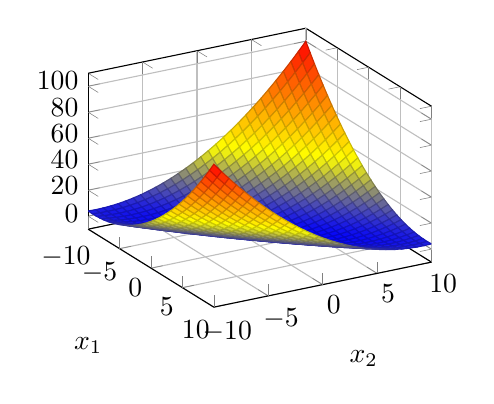
\begin{tikzpicture}
        \begin{axis}[
            xlabel=$x_1$,
            ylabel=$x_2$,
            xtick distance=5,
            ytick distance=5,
            ztick distance=20,
            grid=major,
            %tick style={draw=none},
            domain=-10:10,
            y domain=-10:10,
            view={60}{30},
            width=0.49\textwidth,
        ]
            \addplot3[surf, samples=30] {0.26*(x^2 + y^2) - 0.48*x*y};
        \end{axis}
    \end{tikzpicture}
    }
    \subfloat[Curvas de nivel de la función de Matyas]{
    \begin{tikzpicture}
        \begin{axis}[
            xlabel=$x_1$,
            ylabel=$x_2$,
            xtick distance=2,
            ytick distance=2,
            domain=-10:10,
            y domain=-10:10,
            view={0}{90},
            width=0.49\textwidth,
        ]
        \addplot3[contour gnuplot={
            levels={0, 1, 2, 5, 10, 20, 30, 50},
            labels=false,},
            thick,
            samples=30] gnuplot {0.26*(x**2 + y**2) - 0.48*x*y};
        \end{axis}
    \end{tikzpicture}
    }
    \caption{}
\end{figure}

\noindent Al correr nuestros programas, obtenemos la siguiente tabla:
\begin{table}[H]
    \begin{NiceTabular}{ccccc}[hvlines-except-borders,cell-space-limits=5pt,rules={color=white,width=1pt}]
        \CodeBefore
        \rowcolor{cw0!80}{1}
        \rowcolors{2}{cw2!70!white}{cw1!30!white}
        \Body
        \RowStyle[color=white]{}
        \RowStyle{\bfseries}
        Método & Iteraciones & Punto óptimo & Función evaluada & Error \\
        Máxima Pendiente & $289$ & $\left(-1.6979 \times 10^{-5}, -1.6979 \times 10^{-5}\right)$ & $0.000000$ & $9.7774 \times 10^{-7}$ \\
        Método de Newton & $2$ & $(0.000000, 0.000000)$ & $0.000000$ & $ 0.000000$\\
        Cuasi-Newton Rango 1 & $4$ & $(-0.000000, 0.000000)$ & $0.000000$ & $0.000000$ \\
        Gradientes Conjugados & $268$ & $(0.000000, 0.000000)$ & $0.000000$ & $0.373552$ \\
        Hooke-Jeeves & $42$ & $(-0.000000, -0.000000)$ & $0.000000$ & $0.000000$
    \end{NiceTabular}
    \caption{Resultados de la función de Matyas usando \emph{multistart} con $N = 2500$}
\end{table}

Los métodos \textbf{Método de Newton} y \textbf{Cuasi-Newton Rango 1} convergen de forma casi instantánea, en 2 y 4 iteraciones respectivamente, alcanzando exactamente $(0,0)$ con valor de función nulo y error cero. Esto confirma su gran eficiencia y precisión al resolver funciones cuadráticas suaves.

Por su parte, \textbf{Hooke–Jeeves} también logra converger con total exactitud, aunque requiere 42 iteraciones, lo que indica un coste computacional moderado. El método de \textbf{Máxima Pendiente} precisa 289 iteraciones para aproximarse a $(0,0)$, con un error residual muy bajo, reflejando su eficacia pero un mayor esfuerzo iterativo.

\newpage

En contraste, los \textbf{Gradientes Conjugados} no consiguen situarse exactamente en el óptimo global tras 268 iteraciones, quedando en $(0,0)$ con un elevado error residual. Por tanto, el método de Newton y Cuasi-Newton resultan las opciones más recomendables para la función de Matyas, mientras que Gradientes Conjugados presenta un rendimiento claramente inferior.

\section{Función Three-Hump Camel} % 29

La función de Matyas está definida como:
$$f(\mathbf{x}) = 2x_1^2 - 1.05x_1^4 + \frac{x_1^6}{6} + x_1x_2 + x_2^2.$$
Está función la evaluaremos en $x_i \in [-5, 5]$, para $i = 1, 2$. En \citep{sfuoptimization}, se menciona que el mínimo global está en $\mathbf{x}^* = (0, 0)$ y al evaluarlo en la función se obtiene $f\left(\mathbf{x}^*\right) = 0$.
\begin{figure}[H]
    \centering
    \subfloat[Gráfica de la función Three-Hump Camel]{
    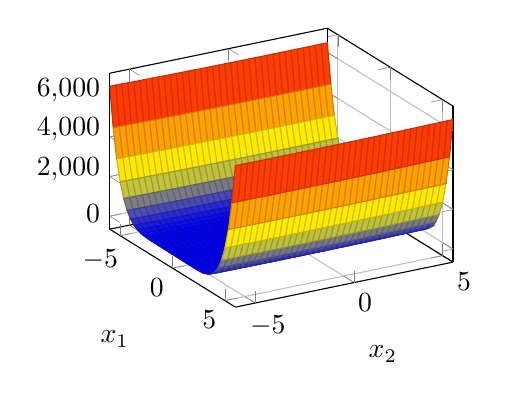
\begin{tikzpicture}
        \begin{axis}[
            xlabel=$x_1$,
            ylabel=$x_2$,
            xtick distance=5,
            ytick distance=5,
            ztick distance=2000,
            grid=major,
            domain=-6:6,
            y domain=-6:5,
            view={60}{30},
            width=0.49\textwidth,
        ]
            \addplot3[surf, samples=37] {2*x^2 - 1.05*x^4 + (x^6)/6 + x*y + y^2};
        \end{axis}
    \end{tikzpicture}
    }
    \subfloat[Curvas de nivel de la función Three-Hump Camel]{
    \begin{tikzpicture}
        \begin{axis}[
            xlabel=$x_1$,
            ylabel=$x_2$,
            xtick distance=5,
            ytick distance=5,
            domain=-5:5,
            y domain=-5:5,
            view={0}{90},
            width=0.49\textwidth,
        ]
        \addplot3[contour gnuplot={
            levels={0, 1, 2, 3, 4, 5, 7, 10, 15, 20},
            labels=false,},
            thick,
            samples=30] gnuplot {2*x**2 - 1.05*x**4 + (x**6)/6 + x*y + y**2};
        \end{axis}
    \end{tikzpicture}
    }
    \caption{}
\end{figure}

\noindent Al correr nuestros programas, obtenemos la siguiente tabla:
\begin{table}[H]
    \begin{NiceTabular}{ccccc}[hvlines-except-borders,cell-space-limits=5pt,rules={color=white,width=1pt}]
        \CodeBefore
        \rowcolor{cw0!80}{1}
        \rowcolors{2}{cw2!70!white}{cw1!30!white}
        \Body
        \RowStyle[color=white]{}
        \RowStyle{\bfseries}
        Método & Iteraciones & Punto óptimo & Función evaluada & Error \\
        Máxima Pendiente &$17$ &$(0.000000, -0.000000)$ & $0.000000$&$0.000005$ \\
        Método de Newton & $4$& $ (0.000000, 0.000000)$& $0.000000$&$0.000000$ \\
        Cuasi-Newton Rango 1 & $5$ & $(0.000000, 0.000000)$ & $0.000000$ & $0.000000$ \\
        Gradientes Conjugados & $4$&$(0.000000, 0.000000)$ & $0.000000$&$ 0.062808$ \\
        Hooke-Jeeves & $53$ & $(0.000000, -0.000000)$ & $0.000000$ & $0.000000$
    \end{NiceTabular}
    \caption{Resultados de la función Three-Hump Camel usando \emph{multistart} con $N = 2500$}
\end{table}

Observamos que el \textbf{Método de Newton} alcanza el óptimo global $(0,0)$ en tan solo 4 iteraciones con error nulo, seguido muy de cerca por el \textbf{Cuasi-Newton Rango 1} en 5 iteraciones, también con precisión perfecta. El método de \textbf{Máxima Pendiente} requiere 17 iteraciones para aproximarse a $(0,0)$ con un error residual mínimo de $5\times10^{-6}$, lo que demuestra un buen equilibrio entre coste iterativo y exactitud.

El método de Hooke–Jeeves converge en 53 iteraciones con error cero, pero requiere más esfuerzo computacional. Los Gradientes Conjugados alcanzan $(0,0)$ en 4 iteraciones, pero con un error elevado de $0.0628$.

En conclusión, para la función Three-Hump Camel, Newton y Cuasi-Newton destacan por su rapidez y exactitud. Máxima Pendiente y Hooke–Jeeves ofrecen soluciones precisas a costa de más iteraciones, mientras que Gradientes Conjugados, pese a su velocidad, pierde precisión y no es recomendable.  

\section{Función de Easom} % 34

La función de Easom está definida como:
$$f(\mathbf{x}) = -\cos(x_1) \cos(x_2) e^{-(x_1 - \pi)^2 - (x_2 - \pi)^2}.$$
Está función la evaluaremos en $x_i \in [-100, 100]$, para $i = 1, 2$. En \citep{sfuoptimization}, se menciona que el mínimo global está en $\mathbf{x}^* = (\pi, \pi)$ y al evaluarlo en la función se obtiene $f\left(\mathbf{x}^*\right) = -1$.
\begin{figure}[H]
    \centering
    \subfloat[Gráfica de la función de Easom]{
    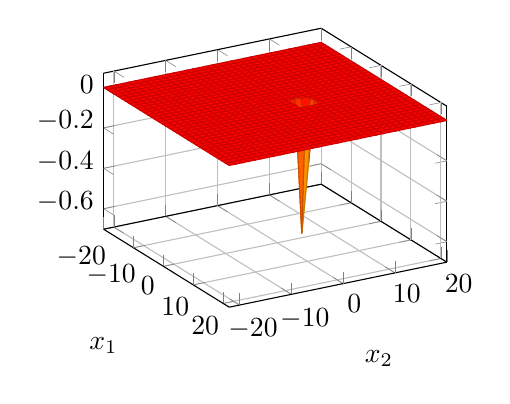
\begin{tikzpicture}
        \begin{axis}[
            xlabel=$x_1$,
            ylabel=$x_2$,
            xtick distance=10,
            ytick distance=10,
            ztick distance=0.2,
            grid=major,
            domain=-20:22,
            y domain=-22:20,
            view={60}{30},
            width=0.49\textwidth,
        ]
            \addplot3[surf, samples=35] {-cos(deg(x)) * cos(deg(y)) * exp(-((x - pi)^2 + (y - pi)^2))};
        \end{axis}
    \end{tikzpicture}
    }
    \subfloat[Curvas de nivel de la función de Easom]{
    \begin{tikzpicture}
        \begin{axis}[
            xlabel=$x_1$,
            ylabel=$x_2$,
            xtick distance=10,
            ytick distance=10,
            domain=-20:20,
            y domain=-20:20,
            view={0}{90},
            width=0.49\textwidth,
        ]
        \addplot3[contour gnuplot={
            levels={-1, -0.8, -0.6, -0.4, -0.2, 0},
            labels=false,},
            thick,
            samples=30] gnuplot {-cos(x)*cos(y)*exp(-((x - pi)**2 + (y - pi)**2))};
        \end{axis}
    \end{tikzpicture}
    }
    \caption{}
\end{figure}

\noindent Al correr nuestros programas, obtenemos la siguiente tabla:
\begin{table}[H]
    \begin{NiceTabular}{ccccc}[hvlines-except-borders,cell-space-limits=5pt,rules={color=white,width=1pt}]
        \CodeBefore
        \rowcolor{cw0!80}{1}
        \rowcolors{2}{cw2!70!white}{cw1!30!white}
        \Body
        \RowStyle[color=white]{}
        \RowStyle{\bfseries}
        Método & Iteraciones & Punto óptimo & Función evaluada & Error \\
        Máxima Pendiente & $0$ & $(-25.092, 90.1429)$ & $0.000000$ & Inf \\
        Método de Newton & $4$ & $(3.141593, 3.141593)$ & $-1.000000$ & $0.000000$ \\
        Cuasi-Newton Rango 1 & $1$ & $(3.859517, 7.948789)$ & $-0.000000$ & $4.860509$ \\
        Gradientes Conjugados & $0$ & $(-4.160045, 19.026372)$ & $0.000000$ & $0.000000$ \\
        Hooke-Jeeves & $49$ & $(3.141593, 3.141593)$ & $-1.000000$ & $0.000000$
    \end{NiceTabular}
    \caption{Resultados de la función de Easom usando \emph{multistart} con $N = 2500$}
\end{table}

\newpage

El Método de Newton alcanza el óptimo global $(\pi,\pi)$ con $f(\pi,\pi)=-1$ en 4 iteraciones, demostrando alta eficiencia. Hooke–Jeeves también converge a $(\pi,\pi)$ y $f=-1$, pero en 49 iteraciones, lo que incrementa el coste computacional. Cuasi-Newton Rango 1 se detiene en $(3.8595,7.9488)$ tras 1 iteración, con $f \approx 4.860509$. Los métodos de Máxima Pendiente y Gradientes Conjugados no progresan: el primero retorna función 0 con error infinito, mientras que el segundo queda en un punto alejado sin mejorar el valor óptimo.

En conclusión, el Método de Newton es la mejor opción para la función de Easom, ya que combina rapidez y exactitud en la búsqueda del mínimo real. Hooke–Jeeves es fiable pero lento, Cuasi–Newton es rápido pero impreciso, y Máxima Pendiente y Gradientes Conjugados no convergen bien.

\section{Función de Beale} % 36

La función de Beale está definida como:
$$f(\mathbf{x}) = (1.5 - x_1 + x_1 x_2)^2 + \left(2.25 - x_1 + x_1 x_2^2\right)^2 + \left(2.625 - x_1 + x_1 x_2^3\right)^2.$$
Está función la evaluaremos en $x_i \in [-4.5, 4.5]$, para $i = 1, 2$. En \citep{sfuoptimization}, se menciona que el mínimo global está en $\mathbf{x}^* = (3, 0.5)$ y al evaluarlo en la función se obtiene $f\left(\mathbf{x}^*\right) = 0$.
\begin{figure}[H]
    \centering
    \subfloat[Gráfica de la función de Beale]{
    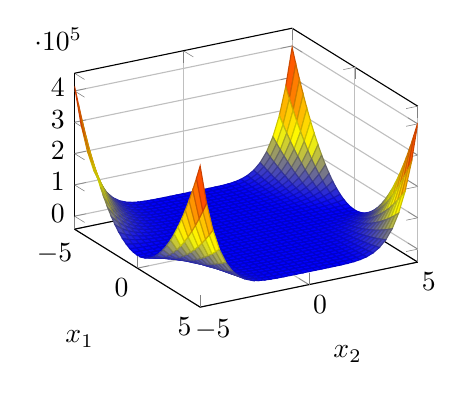
\begin{tikzpicture}
        \begin{axis}[
            xlabel=$x_1$,
            ylabel=$x_2$,
            xtick distance=5,
            ytick distance=5,
            ztick distance=100000,
            grid=major,
            domain=-5:5,
            y domain=-5:5,
            view={60}{30},
            width=0.49\textwidth,
        ]
            \addplot3[surf, samples=35] {(1.5 - x + x*y)^2 +(2.25 - x + x*y^2)^2 + (2.625 - x + x*y^3)^2};
        \end{axis}
    \end{tikzpicture}
    }
    \subfloat[Curvas de nivel de la función de Beale]{
    \begin{tikzpicture}
        \begin{axis}[
            xlabel=$x_1$,
            ylabel=$x_2$,
            xtick distance=5,
            ytick distance=5,
            domain=-5:5,
            y domain=-5:5,
            view={0}{90},
            width=0.49\textwidth,
        ]
        \addplot3[contour gnuplot={
            levels={0.5, 1, 2, 5, 10, 20, 50, 100, 200, 500},
            labels=false,},
            thick,
            samples=30] gnuplot {(1.5 - x + x*y)**2 + (2.25 - x + x*y**2)**2 + (2.625 - x + x*y**3)**2};
        \end{axis}
    \end{tikzpicture}
    }
    \caption{}
\end{figure}

\vspace{-0.1cm}
\noindent Al correr nuestros programas, obtenemos la siguiente tabla:
\begin{table}[H]
    \begin{NiceTabular}{ccccc}[hvlines-except-borders,cell-space-limits=5pt,rules={color=white,width=1pt}]
        \CodeBefore
        \rowcolor{cw0!80}{1}
        \rowcolors{2}{cw2!70!white}{cw1!30!white}
        \Body
        \RowStyle[color=white]{}
        \RowStyle{\bfseries}
        Método & Iteraciones & Punto óptimo & Función evaluada & Error \\
        Máxima Pendiente &$478$ &$(3.000000, 0.500000)$ &$0.000000$ &$0.000000$ \\
        Método de Newton & $11$&$(3.000000, 0.500000)$ &$0.000000$ &$0.000000$ \\
        Cuasi-Newton Rango 1 & $14$ & $(3.000000, 0.500000)$ & $0.000000$ & $0.000000$ \\
        Gradientes Conjugados &$63$ &$(3.000000, 0.500000)$ &$0.000000$ &$0.048560$ \\
        Hooke-Jeeves & $61$ & $(3.000000, 0.500000)$ & $0.000000$ & $0.000000$
    \end{NiceTabular}
    \caption{Resultados de la función de Beale usando \emph{multistart} con $N = 2500$}
\end{table}

\newpage

Los métodos \textbf{Método de Newton} y \textbf{Cuasi-Newton Rango 1} destacan por su rapidez y exactitud: convergen al óptimo global $(3,0.5)$ en apenas 11 y 14 iteraciones, respectivamente, logrando valor de función cero y error residual nulo.

El \textbf{Hooke–Jeeves} también alcanza la solución exacta con error cero, aunque requiere 61 iteraciones, mientras que los \textbf{Gradientes Conjugados} tardan 63 iteraciones y presentan un error residual de $0.04856$, lo que revela menor fiabilidad en la convergencia.

Por último, \textbf{Máxima Pendiente} resulta el menos eficiente, necesitando 478 iteraciones para converger exactamente a $(3,0.5)$. En conclusión, Método de Newton y Cuasi-Newton Rango 1 son las opciones más recomendables para la función de Beale, seguidos por Hooke–Jeeves; Gradientes Conjugados y Máxima Pendiente muestran desventajas por su error o coste computacional elevado.

